\chapter{Methods}

% \section{Tracking \& Matching}
% We track the predicted staff and patients across multiple frames, indicated by $t = 1 \ldots T$, by iteratively assigning the predictions, $\{ P_i^{(t)} \}_{i=1}^{M_t}$, to the latest known tracks, $\{ Q^{(t)}_{j} \}_{j=1}^{N_t}$ by greedily picking the assignment with the minimum cost:
% \begin{equation}
%     \argmin_{i,j} \mathcal{L}_\text{track}(P^{(t)}_i, Q^{(t-1)}_j),
% \end{equation}
% until either all predictions or latest tracks have been assigned exactly once. In the case of any unassigned predictions, a new track is initialized. After tracks have been assigned, the latest track $Q^{(t)}_j$ is updated with the assigned predictions. We choose the following composite loss function:
% \begin{equation}
%     \mathcal{L}_\text{track}(P, Q) = \alpha \norm{P_\text{3D kpts} - Q_\text{3D kpts}}{2} + \beta \norm{P_\text{class} - Q_\text{class}}{\infty},
% \end{equation}
% incorporating both the Euclidean distance between the 3D joint keypoints as well as the predicted person class (staff/patient), with $\alpha$ and $\beta$ weighting the influence of each term. The tracks, $T_i$, are then greedily matched to the ground truth annotations $G_j$, minimizing the loss:
% \begin{equation}
%     \mathcal{L}_\text{match}(T, G) = \sum_t^{T} \begin{cases}
%         \norm{a^{(t)}_{\text{track}, \text{2D kpts}} - b^{(t)}_{\text{track}, \text{2D kpts}}}{2} & \text{if}\ a^{(t)}_\text{track} \in a_\text{track} \\
%         \gamma & \text{otherwise}
%     \end{cases}
% \end{equation}
% over the trajectory time horizon $t = 1,2,\ldots,T$ where $\gamma$ is the punishment for not detecting the person.



\section{3D scene reconstruction}
% Two approaches 

% First approach:
% First uses the relative depth disparity maps and the rendered SMPL poses in order to restore the 
% metric depth scale and offset.
% Pros:
% - Relative depth maps are often more accurate and easier for a model to learn.
% Cons:
% - The process of restoring scale and offset is not very robust and can be prone to errors if the SMPL poses don't overlap precisely with the predicted depths.  
% - The reliance of poses at different distances in order to optimally regress the scale and offset parameters.

% Second approach:
% Using metric depth estimation
% Pros:
% - Doesn't rely on rendering SMPL poses and restoring scale and offset.
% - Domain is contained to indoor hospital and carehome rooms.
% Cons:
% - Less accurate predictions

\subsection*{Extracting SMPL poses}
\begin{figure}[H]
    \centering
    \includegraphics[width=\linewidth]{figures/pose-extraction.pdf}
    \caption{Illustration of pose extraction process with occlusion handling.}
    \label{fig:pose-extraction}
\end{figure}
We leverage the pretrained HMR2.0 model from \cite{goel2023humans} for pose extraction, applying it frame-wise to crops of each human bounding box in the frame. This approach ensures proper alignment with existing dataset annotations without the need for additional tracking. To handle potential occlusions that may cause duplicate predictions of the occluding pose, pairwise euclidean keypoint distances are computed for all edges in the bipartite graph of annotated 2D keypoints and SMPL joint 2D projections for individuals in the current frame. Poses with the minimum keypoint distance to other individuals' annotated keypoints are masked out.


% TODO: Write something about the annotations in the Teton data section.


\subsection*{Restoring scene depth}
We combine both metric and relative variants of the Depth Anything model (\cite{depthanything}) to restore the depth of the scene. Using the low-resolution 384x512 metric depth predictions, $m_{1:K}$ (upsampled to match higher resolution disparity maps), we restore the scaling and offset from the higher resolution predicted disparity maps, $d_{1:K}$, by linearly fitting the disparity scaling $\alpha$ and offset $\beta$ according to $\argmin \alpha \cdot d_{1:K} + \beta - 1 / m_{1:K}$ for all $K$ key frames to get our upscaled metric depths, $m^*_{1:K} := 1 / (\alpha \cdot d_{1:K} + \beta)$.

% TODO: We are assuming that the relative doesn't change dynamic range during the scene (which might be wrong). Save for discussion.


% We utilize pseudo ground truth disparity maps generated by the Depth Anything model, inversely proportional to the scene depth, in order to reconstruct a point cloud of the scene. To recover the depth scale and offset we rasterize the predicted SMPL poses, extract the z-buffer, compute the inverse depth and regress the intersection with the normalized disparity maps using the Random Sample Consensus (RANSAC) algorithm robust to outliers. 

% \begin{equation}
%     \begin{bmatrix}p
%         x \\ y \\ 1/z \\ 1
%     \end{bmatrix} = \begin{bmatrix}
%         f_x & 0 & 0 & p_x \\
%         0 & f_y & 0 & p_y \\
%         0 & 0 & 1 & 0 \\
%         0 & 0 & 0 & 1
%     \end{bmatrix} \begin{bmatrix}
%         X \\ Y \\ Z \\ 1
%     \end{bmatrix}
% \end{equation}


% \begin{equation}
%     X = \frac{Z}{f_x} \left( x - p_x \right) , \quad Y = \frac{Z}{f_x} \left(y - p_y \right)
% \end{equation}
% where $f_x$, $f_y$ are the horizontal and vertical focal lenghts respectively and ($p_x$, $p_y$) is the principal point often chosen as the center $(w/2,h/2)$ of the image. 

\section{Human pose sequence optimization}
Due to poses being predicted independently per frame, the combined pose sequences often lack temporal consistency, resulting in janky or erratic movements. To address this issue, we refine the pose sequences by optimizing for smooth trajectories across all $1 \dots T$ frames by minimizing a composite smooth loss objective assuming constant velocity:

\begin{equation}
    \mathcal{L}_\text{smooth} = \sum_t{\| \hat{\vect{\tau}}^{(t)} - \vect{\tau}^{(t)} \|_2} + \lambda_{\hat{\tau}} \sum_t{\mathcal{R}_{\bar{\tau}}^{(t)}}
\end{equation}

where $\hat{\vect{\tau}}^{(t)} = \vect{\tau}^{(t-1)} + \vect{v}^{(t-1)}$ is the predicted location at time $t$ assuming constant velocity $\vect{v}^{(t)} = \vect{\tau}^{(t)} - \vect{\tau}^{(t-1)}$, and $\mathcal{R}_{\bar{\tau}}^{(t)} = \| \vect{\tau}^{(t)} - \bar{\vect{\tau}}^{(t)} \|_2$ a regularization term preventing the optimized location $\mathbf{\tau}^{(t)}$ to not diverge too far from the initially predicted location $\bar{\vect{\tau}}^{(t)}$.



% Something about using the original poses + vPoser (human pose prior) + annotated keypoints.
% TODO: Write this?


\section{Unification of datasets}
Before concatenating the HumanML3D, InterHuman and our own Teton dataset we make sure they all conform to the same coordinate system and scaling by implicitly representing the floor as the XY-plane with positive Z indicating the upwards direction using metric units for coordinates. This removes the need to explicitly condition the model on the floor plane possibly simplifying the learning task for more efficient training.


\subsection*{Aligning floor with XY-plane}
\begin{figure}[H]
    \centering
    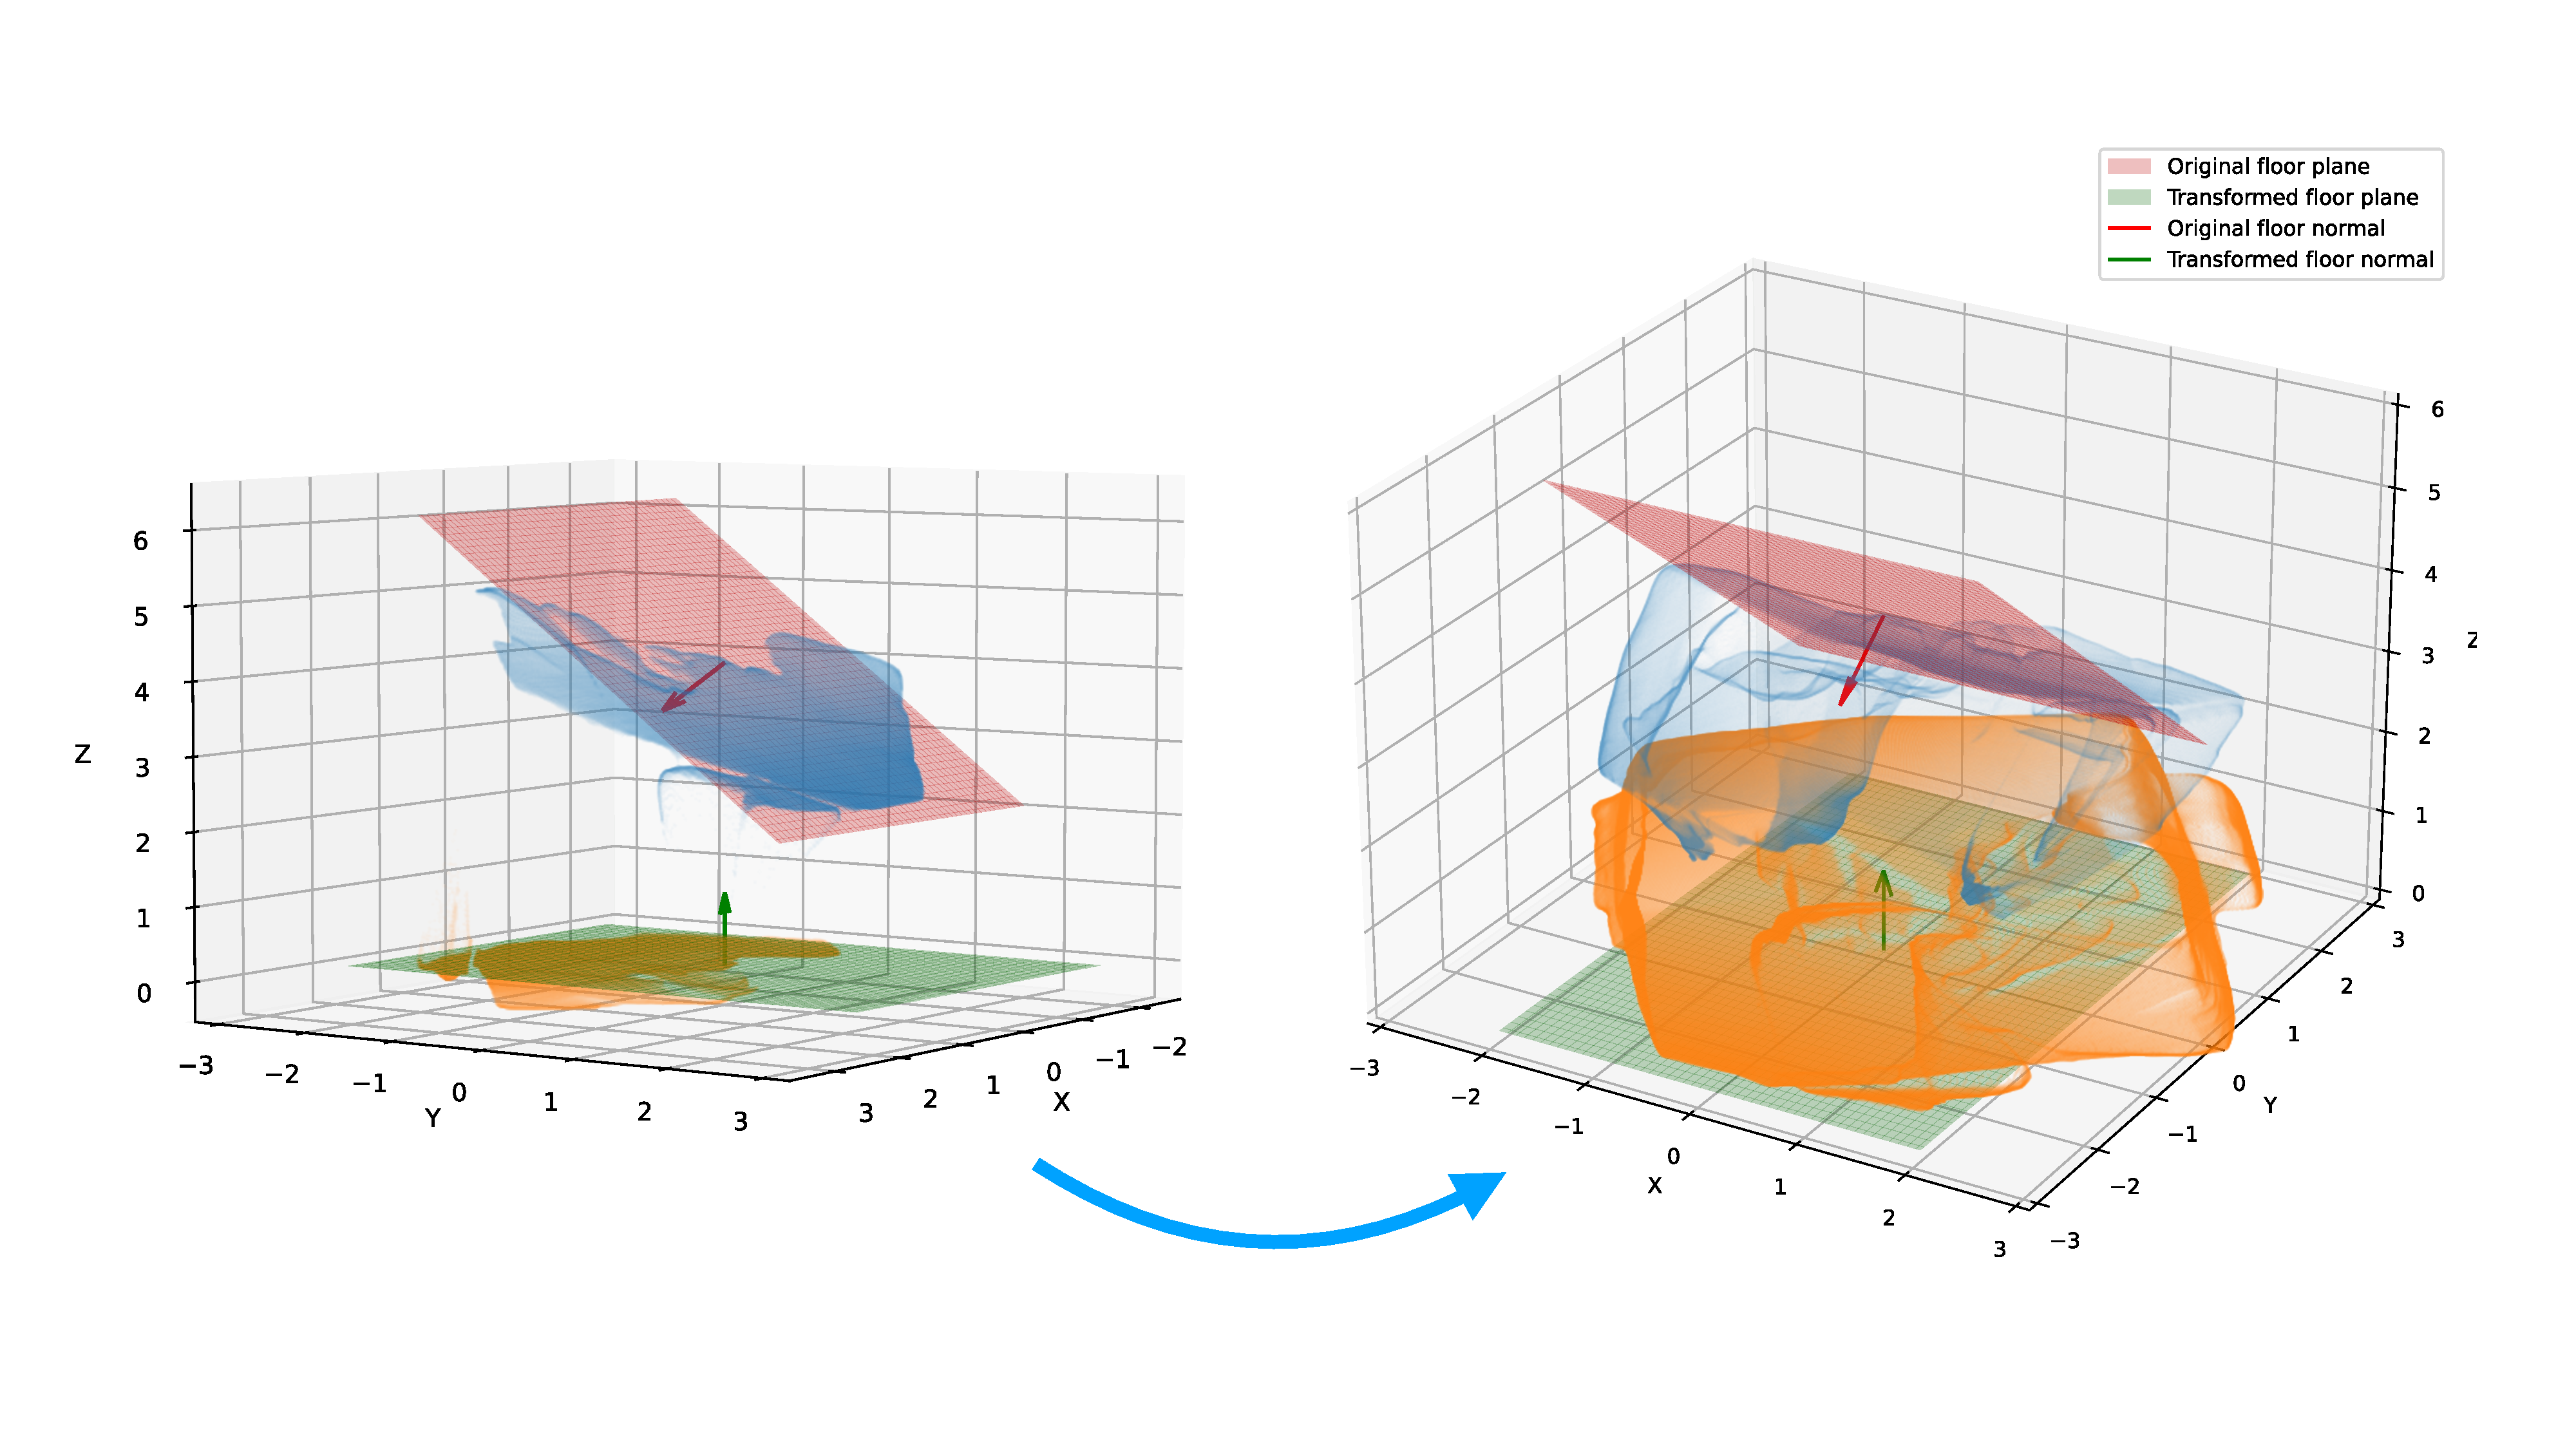
\includegraphics[width=\linewidth]{figures/rotation.pdf}
    \caption{Translation and rotation of room point cloud aligning the floor with the XY-plane.}
    \label{fig:rotate-floor-planes}
\end{figure}

Using the floor segmentation masks we isolate the floor point cloud and use the outlier robust RANSAC regressor with inline threshold of 10cm to fit the plane equation:

\begin{equation}
    z = \beta_z + \beta_x x + \beta_y y
\end{equation}


To compute the rotation matrix that aligns the normal vector $\hat{\vect{n}}_\text{floor} = \vect{n}_\text{floor} / \| \vect{n}_\text{floor} \|$ (where $\vect{n}_\text{floor} = (0, 1, b_y)^T \times (1, 0, b_x)^T$) of the floor plane in the camera coordinate system with the normal vector $\vect{n}_{XY} = (0, 0, 1)$ of the XY-plane, we can utilize Rodrigues' rotation formula. 

First, we construct the skew-symmetric matrix $\mathbf{K}$ from the components of the cross product vector $\vect{v} = \hat{\vect{n}}_\text{floor} \times \vect{n}_{XY}$. The skew-symmetric matrix $\mathbf{K}$ is defined as:
\begin{equation}
    \mathbf{K} = \begin{bmatrix}
        0 & -v_3 & v_2 \\
        v_3 & 0 & -v_1 \\
        -v_2 & v_1 & 0
    \end{bmatrix}
\end{equation}

Next, we compute the rotation matrix $\mathbf{R}$ using Rodrigues' rotation formula. The formula incorporates the identity matrix $\mathbf{I}$, the skew-symmetric matrix $\mathbf{K}$, and a scaling term based on the angle between the vectors. The resulting rotation matrix is given by:

\begin{equation}
    \mathbf{R} = \mathbf{I} + \mathbf{K} + \mathbf{K}^2 \left(\frac{1 - c}{s^2}\right)
\end{equation}

Here, $\mathbf{I}$ is the identity matrix, $c$ is the dot product of $\mathbf{a}$ and $\mathbf{b}$, and $s$ is the norm of the cross product vector $\mathbf{v}$. This formula ensures that the rotation matrix $\mathbf{R}$ not only aligns $\mathbf{a}$ with $\mathbf{b}$ but also preserves the orthogonality and orientation of the coordinate system.

Finally, we transform the point cloud by translating it to align the floor plane intercept with the origin, followed by rotating it using the computed rotation matrix:

\begin{equation} \label{eq:transform-points}
    \vect{p}^* = \mathbf{R} \left(\vect{p} - (0, 0, b_z)^T \right) 
\end{equation}
In a similar fashion, we transform our poses by applying \cref{eq:transform-points} to our pose root joint translations. Since our joint rotations are relative to the root global orientation, $\mathbf{O}$, we first compute its inverse global-to-local rotation matrix, $\mathbf{O}^{-1}$. After applying the new rotation matrix $\mathbf{R}$, we then invert the result to convert back from local-to-global orientation:

\begin{equation}
    \mathbf{O}^* = \left(\mathbf{R} \mathbf{O}^{-1} \right)^{-1}
\end{equation}
The resulting transformation of the point cloud and poses in aligning the floor with the XY-plane is illustrated in \cref{fig:rotate-floor-planes}.

\section{Motion and scene representation}
Previous work on single human motion generation uses a canonical representation 

% We use a 6D continuous representation of the joint angles as according to \cite{Zhou_2019_CVPR}.
% We represent the motion similar to 


\section{Diffusion model}



